\chapter{Testes de Usabilidade}

Uma das definições mais encontradas na literatura é a de que a usabilidade é parte de um projeto mais amplo, que aponta para o desenvolvimento de métodos e técnicas que podem incorporar considerações de ergonomia dentro do processo de design e avaliação da interface homem/computador \cite{bastien1993ergonomic}. A ISO/IEC FCD 9126-1 define usabilidade como a capacidade do software ser compreendido, aprendido, usado e apreciado pelo usuário, dado as condições específicas \cite{gonccalves2009usabilidade}.

As experiências negativas no uso de interfaces frustam os usuários, fazendo com que se sintam diminuído, culpando-se por não conseguir realizar tarefas que, hipoteticamente, outros usuários conseguem \cite{gonccalves2009usabilidade}. Quando essa dificuldade é frequente a frustração pode levar o usuário ao estresse e ansiedade, devido à sequência de experiências negativas \cite{cybis2003engenharia}.

Para que a revolução digital ocorra, um computador deve representar-se ao usuário, numa linguagem que este compreenda, por isso, os sistemas computacionais precisam utilizar elementos na interface que sejam intuitivos e de fácil compreensão para que o usuário consiga atingir seus objetivos \cite{johnson2001cultura}.

Portanto, foi levado em consideração técnicas de UI e UX durante todo o desenvolvimento das aplicações WEB e Mobile com o objetivo de facilitar a usabilidade e deixar a experiência mais fluida possível para o usuário, evitando com que haja frustrações para com o sistema desenvolvido.

\subsection{Elaboração dos Testes Aplicados}

A usabilidade é uma qualidade de uso, ou seja, ela é definida ou medida para um determinado contexto no qual um sistema é operado. Assim, um sistema pode proporcionar boa usabilidade para um usuário experiente, mas péssima para um iniciante, ou vice-versa, ou ainda, pode ser fácil operar se o sistema for usado esporadicamente, mas difícil se for utilizado frequentemente \cite{cybis2003engenharia}.

Para isso, estudos como os de \cite{bastien1993ergonomic}, apresentam regras e recomendações para que os sistemas computacionais sejam elaborados de modo a facilitar sua aprendizagem e uso, proporcionando usabilidade.

Para a avaliação do projeto, foi elaborado uma metodologia de verificação de alguns requisitos visando a análise e a usabilidade padrão mínimo para a implantação e utilização do web/mobile. Para isso foi criado algumas situações de usabilidade segundo alguns trabalhos científicos como a de \cite{silva2016principios}, onde verifica-se alguns critérios importantes que foram formulados para a aplicação das avaliações do desenvolvimento dos projetos Integradores. As avaliações aconteceram de forma remota com uma amostragem de aproximadamente 19 usuários, incluindo os colaboradores da empresa Duas Rodas.

Para a elaboração dos resultados, foram realizadas as médias de todas as avaliações e unificadas graficamente, buscando descreve-las o mais transparente possível. Para isso, foi criado 3 módulos de avaliação que são eles: Critério Geral de Apresentação, Critérios Gerais e Erros Comuns, onde respectivamente encontra-se como características de \textit{layout}, características de desenvolvimento e erros que podem ocorrer no projeto.

\subsection{Discussão dos Resultados}

Verificou-se no Gráfico \ref{criterio-geral-apresentacao} de Critérios Gerias de apresentação do projeto Agil.It que o percentual de avaliação teve um aproveitamento de 84,5\% e média de todos os resultados avaliados de 8,5, considerando os critérios de apresentação dos \textit{layouts}, onde as notas foram de 1-10 avaliando cada quesito, como observa-se no gráfico.

\begin{landscape}
\begin{figure}[H]
	\caption{\label{criterio-geral-apresentacao}Critério Geral de Apresentação}
	\begin{center}
		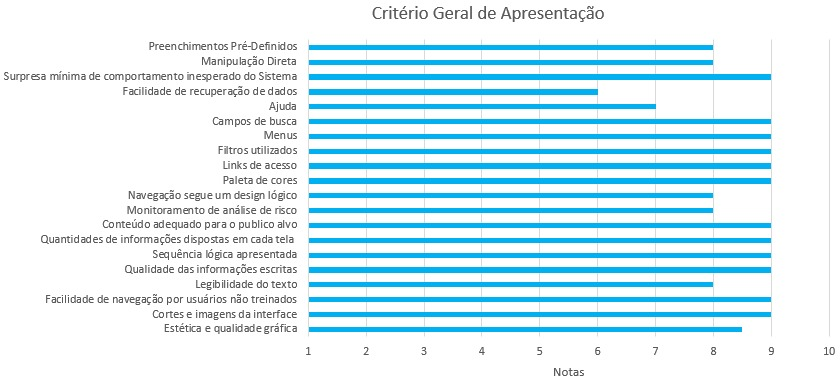
\includegraphics[scale=0.90]{./Figuras/cap-testes/criterio-geral-apresentacao.jpeg}
	\end{center}
\end{figure}
\end{landscape}

Para a análise dos Critérios Gerais, observa-se no gráfico \ref{criterios-gerais} que o foco principal foi no desenvolvimento e desempenho do software considerando características fundamentais para o sucesso da usabilidade e da aprovação do Usuário. Neste quesito, a avaliação ficou em um aproveitamento de 88,2\% com a média de 8,8 dos quesitos avaliados.

\begin{figure}[H]
	\caption{\label{criterios-gerais}Critérios Gerais}
	\begin{center}
		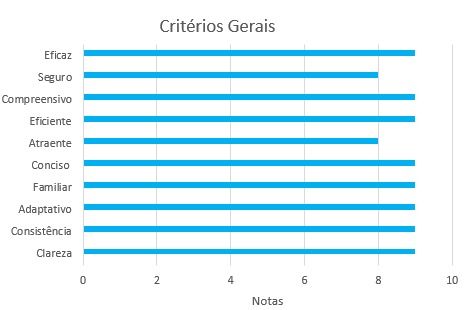
\includegraphics[scale=0.86]{./Figuras/cap-testes/criterios-gerais.jpeg}
	\end{center}
\end{figure}

Quanto a avaliação dos Erros Comuns, foi avaliado com aplica-se ou não este quesito, e observa-se na tabela \ref{percentual-medio-aprovacao} que, o software de gerenciamento do Agil.It, chegou a um percentual médio de aprovação de 92\%, sendo assim, considera-se ótimo o percentual obtido na avaliação, na etapa do projeto.

\begin{table}[H]
	\caption{\label{percentual-medio-aprovacao}Percentual Médio de Aprovação em Erros Comuns de Usabilidade}
	\begin{tabular}{|l|c|l|l|l|l|l|}
		\hline
		\rowcolor[HTML]{656565} 
		& \multicolumn{5}{c|}{\cellcolor[HTML]{656565}{\color[HTML]{FFFFFF} \textbf{Erros   comuns de Usabilidade}}} & \multicolumn{1}{c|}{\cellcolor[HTML]{656565}{\color[HTML]{FFFFFF} \textbf{\begin{tabular}[c]{@{}c@{}}Percentual\\ Médio\\ Aprovação\end{tabular}}}} \\ \hline
		1                        & \multicolumn{5}{c|}{Ícones   e Menus ambíguos}                                                             &                                                                                                                                                        \\ \cline{1-6}
		2                        & \multicolumn{5}{c|}{Linguagens   que permitem apenas movimentos direcionados de forma única}               &                                                                                                                                                        \\ \cline{1-6}
		3                        & \multicolumn{5}{c|}{Limite   de entrada e manipulação}                                                     &                                                                                                                                                        \\ \cline{1-6}
		4                        & \multicolumn{5}{c|}{Limite   de seleção e destaque}                                                        &                                                                                                                                                        \\ \cline{1-6}
		5                        & \multicolumn{5}{c|}{Sequência   não clara de passos}                                                       &                                                                                                                                                        \\ \cline{1-6}
		6                        & \multicolumn{5}{c|}{Mais   passos para gerenciar a interface do que para realizar tarefas}                 &                                                                                                                                                        \\ \cline{1-6}
		7                        & \multicolumn{5}{c|}{Links   complexos entre/com aplicações}                                                &                                                                                                                                                        \\ \cline{1-6}
		8                        & \multicolumn{5}{c|}{Confirmações   e Feedbacks inadequados}                                                &                                                                                                                                                        \\ \cline{1-6}
		9                        & \multicolumn{5}{c|}{Pouca   inteligência e antecipação por conta do sistema}                               &                                                                                                                                                        \\ \cline{1-6}
		10                       & \multicolumn{5}{c|}{Mensagem   de erro, tutoriais ajuda e documentação inadequadas}                        &                                                                                                                                                        \\ \cline{1-6}
		\multicolumn{1}{|c|}{11} & \multicolumn{5}{c|}{Poluição Visual}                                                                       &                                                                                                                                                        \\ \cline{1-6}
		\multicolumn{1}{|c|}{12} & \multicolumn{5}{c|}{Má Organização da Informação}                                                          &                                                                                                                                                        \\ \cline{1-6}
		\multicolumn{1}{|c|}{13} & \multicolumn{5}{c|}{Componentes Incompreensíveis}                                                          &                                                                                                                                                        \\ \cline{1-6}
		\multicolumn{1}{|c|}{14} & \multicolumn{5}{c|}{Distrações irritantes}                                                                 &                                                                                                                                                        \\ \cline{1-6}
		\multicolumn{1}{|c|}{15} & \multicolumn{5}{c|}{Navegação Ineficiente}                                                                 &                                                                                                                                                        \\ \cline{1-6}
		\multicolumn{1}{|c|}{16} & \multicolumn{5}{c|}{Sobrecarga de Informações}                                                             & \multirow{-16}{*}{92\%}                                                                                                                                \\ \hline
	\end{tabular}
	\legend{Fonte: os autores (2020)}
\end{table}